\documentclass[10pt,a4paper]{article}
\usepackage[utf8]{inputenc}
\usepackage[english]{babel}
\usepackage[T1]{fontenc}
\usepackage[a4paper,top=2.54cm,bottom=2.54cm,left=3.17cm,right=3.17cm]{geometry}
\usepackage{graphicx}
\usepackage[plainpages=false,pdfauthor={Generated with SB pipe},pdftitle={Report: insulin receptor stoch (Time Courses Task)},pdftex]{hyperref}
\hypersetup{colorlinks=false,linkcolor=blue}
\usepackage{url}
\usepackage{makeidx}
\author{A clever scientist} 
\title{Report: insulin receptor stoch}
\date{\today}
\makeindex
\begin{document}
\maketitle
\begin{abstract}
Time Courses Task\end{abstract}
\tableofcontents
\section{Simulation}
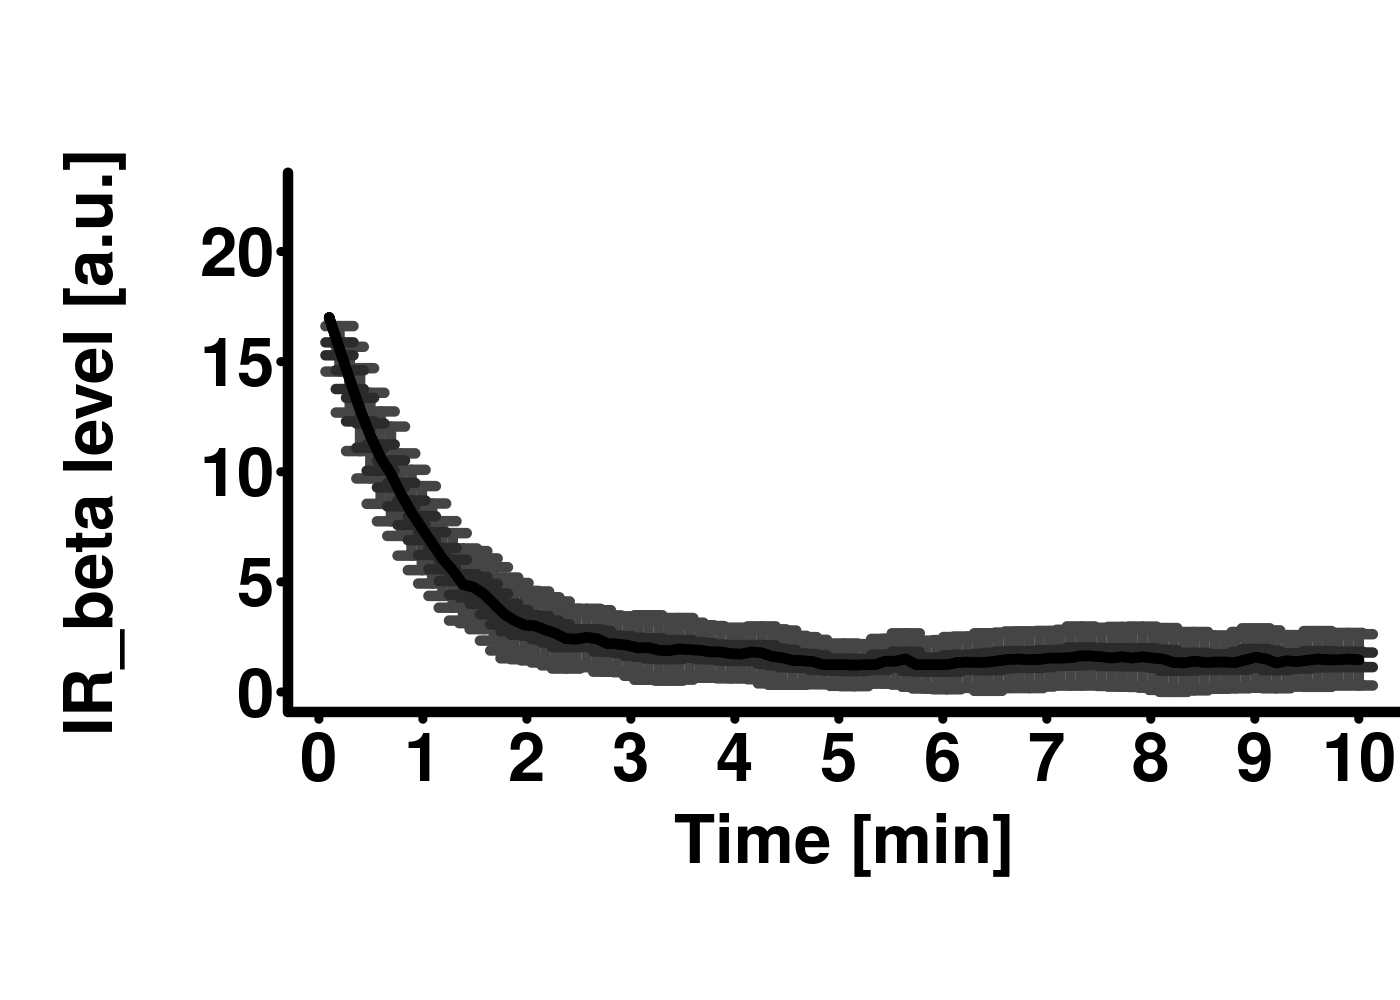
\includegraphics[scale=0.08]{plots_stoch_tc_mean/insulin_receptor_stoch_sd_n_ci95_IR_beta.png}
\hfill
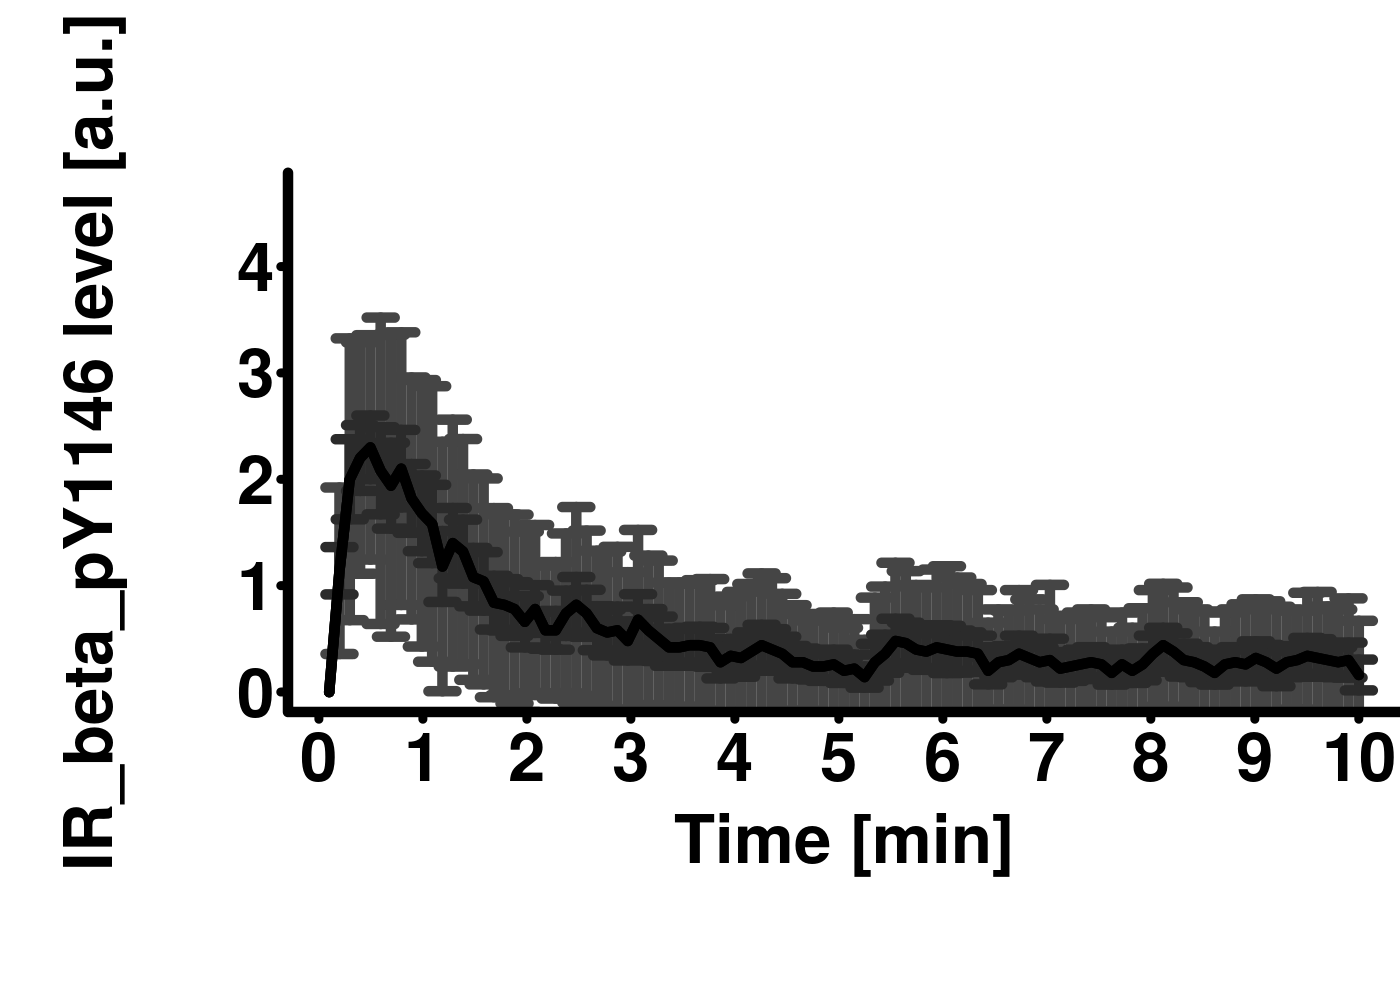
\includegraphics[scale=0.08]{plots_stoch_tc_mean/insulin_receptor_stoch_sd_n_ci95_IR_beta_pY1146.png}
\hfill
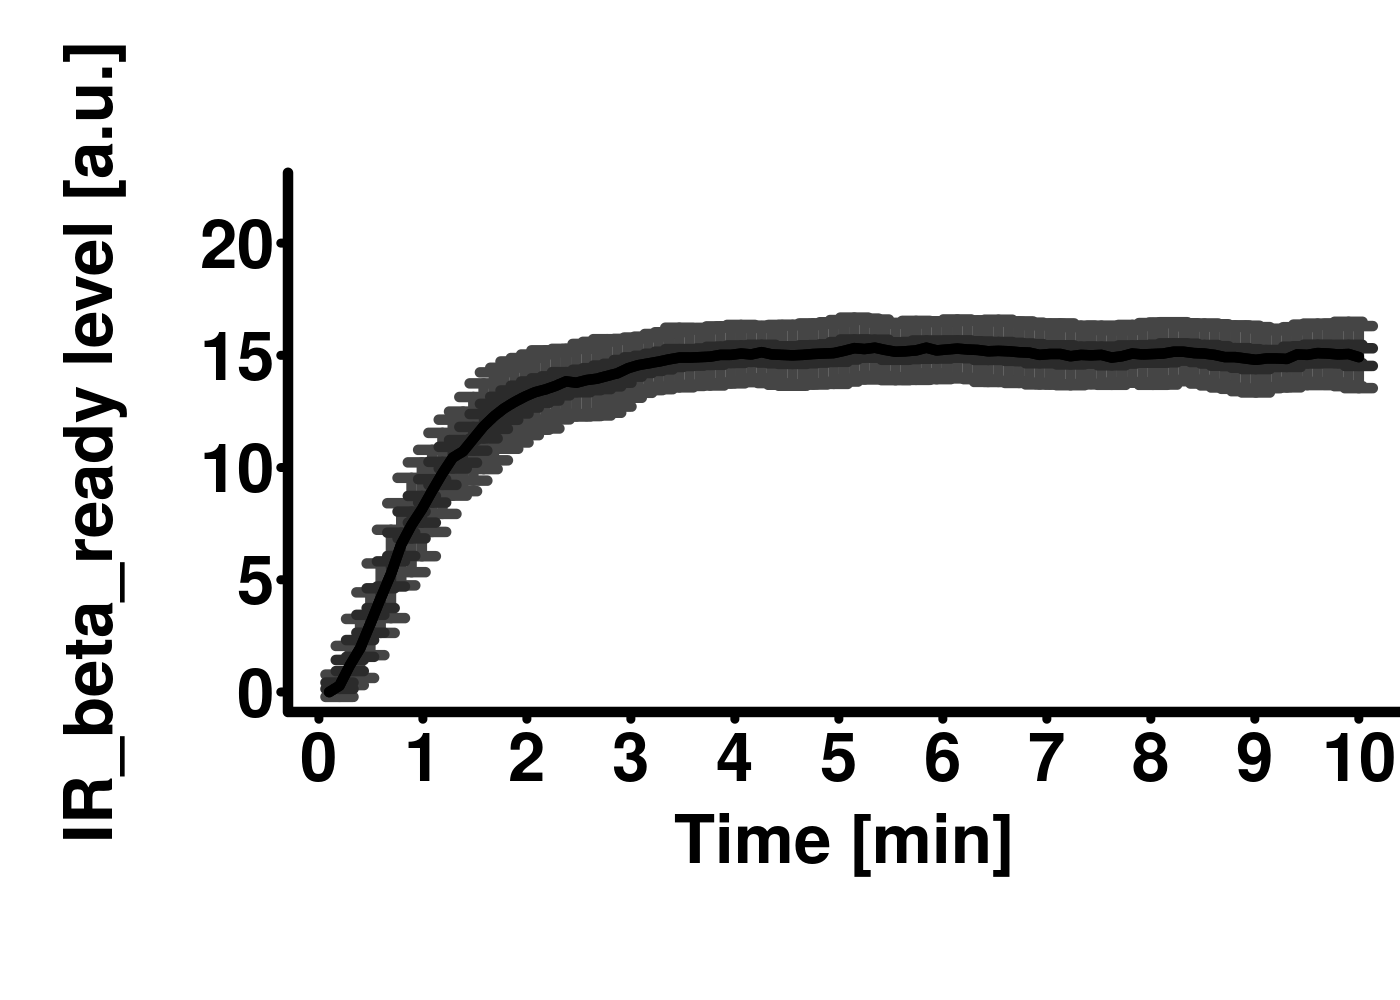
\includegraphics[scale=0.08]{plots_stoch_tc_mean/insulin_receptor_stoch_sd_n_ci95_IR_beta_ready.png}
\hfill
\end{document}
